\let\negmedspace\undefined
\let\negthickspace\undefined
\documentclass[journal]{IEEEtran}
\usepackage[a5paper, margin=10mm, onecolumn]{geometry}
\usepackage{tfrupee} 
\setlength{\headheight}{1cm} 
\setlength{\headsep}{0mm}     

\usepackage{gvv-book}
\usepackage{gvv}
\usepackage{cite}
\usepackage{amsmath,amssymb,amsfonts,amsthm}
\usepackage{algorithmic}
\usepackage{graphicx}
\usepackage{textcomp}
\usepackage{xcolor}
\usepackage{txfonts}
\usepackage{listings}
\usepackage{enumitem}
\usepackage{mathtools}
\usepackage{gensymb}
%\usepackage{wasysym}
\usepackage{comment}
\usepackage[breaklinks=true]{hyperref}
\usepackage{tkz-euclide} 
\usepackage{listings}
\def\inputGnumericTable{}                                 
\usepackage[latin1]{inputenc}                                
\usepackage{color}                                            
\usepackage{array}                                            
\usepackage{longtable}                                       
\usepackage{calc}                                             
\usepackage{multirow}                                         
\usepackage{hhline}                                           
\usepackage{ifthen}                                           
\usepackage{lscape}
\usepackage{circuitikz}
\tikzstyle{block} = [rectangle, draw, fill=blue!20, 
    text width=4em, text centered, rounded corners, minimum height=3em]
\tikzstyle{sum} = [draw, fill=blue!10, circle, minimum size=1cm, node distance=1.5cm]
\tikzstyle{input} = [coordinate]
\tikzstyle{output} = [coordinate]
\renewcommand{\thefigure}{\theenumi}
\renewcommand{\thetable}{\theenumi}
\setlength{\intextsep}{10pt} % Space between text and floats
\numberwithin{equation}{enumi}
\numberwithin{figure}{enumi}
\renewcommand{\thetable}{\theenumi}

\begin{document}

\bibliographystyle{IEEEtran}
\vspace{3cm}

\title{10.7.81}
\author{EE25BTECH11032 - Kartik Lahoti}
\maketitle

\subsection*{Question: } 
Two circles, each of radius $5$ units, touch each other at $\brak{1,2}$. If the equation of common tangent is 4x + 3y = 10, find the equations of circles.

\textbf{Solution}:\\

Let , 
\begin{align}
    \vec{P} = \myvec{1\\2}
\end{align}


Given Line, 

\begin{align}
    \vec{n}^{\top}\vec{x} = 10
\end{align}

Normal Vector $\vec{n} = \myvec{4 \\ 3}$

Unit vector $\vec{u}$ in direction of $\vec{n}$

\begin{align}
    \vec{u} = \frac{\vec{n}}{\norm{\vec{n}}} = \myvec{\dfrac{4}{5} \\ \dfrac{3}{5}}
\end{align}

Let $\vec{O_i}$ be the center of Circles, then

\begin{align}
    \vec{O_i} = \vec{P} \pm 5\vec{u} \\ 
    \vec{O_i} = \myvec{1\pm4 \\ 2\pm3} 
\end{align} 


\begin{align}
    \therefore \vec{O_1} = \myvec{5 \\ 5} , \vec{O_2} = \myvec{-3\\-1}
\end{align}

Equation of Circles are : 

\begin{align}
    O_1 \colon g\brak{\vec{x}} = \vec{x}^{\top}\vec{V}\vec{x} + 2\vec{u}^{\top}\vec{x} + f 
\end{align}

\begin{table}[H]
    \centering
    \begin{tabular}[12pt]{ |c| c|}
    \hline
    \textbf{Points} & \textbf{Name}\\ 
    \hline
	\myvec{7\\10} & Point $\Vec{A}$ \\
    \hline 
	\myvec{-2\\5} & Point $\Vec{B}$\\
    \hline
	\myvec{3\\4} & Point $\Vec{C}$\\
    \hline
\end{tabular}
    \caption*{}
    \label{tab:placeholder}
\end{table}

\begin{align}
    O_2 \colon g\brak{\vec{x}} = \vec{x}^{\top}\vec{V}\vec{x} + 2\vec{u}^{\top}\vec{x} + f 
\end{align}

\begin{table}[H]
    \centering
    \begin{table}[h!]
    \centering
    \begin{tabular}{|c|c|c|}
        \hline
        Point & For $k=3$ & For $k=-\tfrac{9}{2}$ \\
        \hline
        $A$ & $\myvec{1\\-1}$ & $\myvec{1\\-1}$ \\
$B$ & $\myvec{-4\\6}$ & $\myvec{-4\\-9}$ \\
$C$ & $\myvec{-3\\-5}$ & $\myvec{\tfrac{9}{2}\\-5}$ \\
        \hline
    \end{tabular}
    \caption{Vertices of $\triangle ABC$ after substituting $k$ values}
    \label{tab:triangle_values}
\end{table}

    \caption*{}
    \label{tab:placeholder}
\end{table}

\begin{figure}[H]
    \centering
    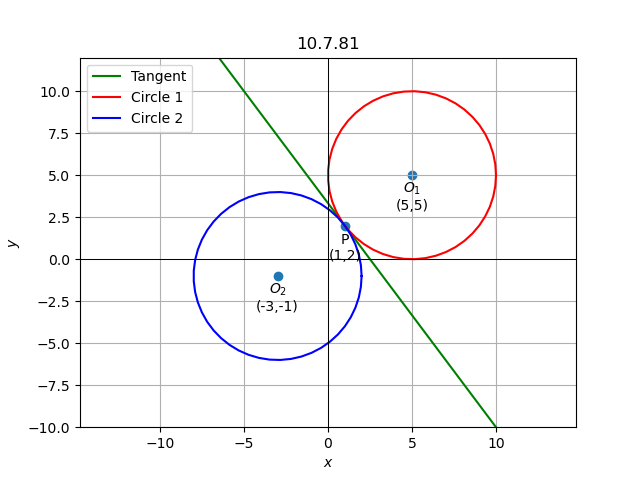
\includegraphics[width=1\columnwidth]{figs/graph2.png}
    \caption*{}
    \label{fig:placeholder}
\end{figure}

\end{document}


